% Author: Nelson Lago
% This file is distributed under the MIT Licence

%%%%%%%%%%%%%%%%%%%%%%%%%%%%%%%%%%%%%%%%%%%%%%%%%%%%%%%%%%%%%%%%%%%%%%%%%%%%%%%%
%%%%%%%%%%%%%%%%%%%%%%%%%%%%%%%%% PREÂMBULO %%%%%%%%%%%%%%%%%%%%%%%%%%%%%%%%%%%%
%%%%%%%%%%%%%%%%%%%%%%%%%%%%%%%%%%%%%%%%%%%%%%%%%%%%%%%%%%%%%%%%%%%%%%%%%%%%%%%%

% A língua padrão é a última da lista
\documentclass[a1paper,brazilian,english]{article}

% Vários pacotes e opções de configuração genéricos
\usepackage{imegoodies}
\usepackage{graphicx}
\usepackage{caption}
\usepackage[poster,hidelinks]{imelooks}
% \tcbposterset{fontsize = 32pt} % default, mude se necessário

% Diretórios onde estão as figuras; com isso, não é necessário (mas
% é permitido) colocar o caminho completo em \includegraphics. Note
% que a extensão nunca é necessária (mas é permitida), ou seja, o
% resultado é o mesmo com "\includegraphics{figuras/foto.jpeg}",
% "\includegraphics{foto.jpeg}", "\includegraphics{figuras/foto}"
% ou "\includegraphics{foto}".
\graphicspath{{figuras/},{fig/},{logos/},{img/},{images/},{imagens/}}

% Comandos rápidos para mudar de língua:
% \en -> muda para o inglês
% \br -> muda para o português
% \texten{blah} -> o texto "blah" é em inglês
% \textbr{blah} -> o texto "blah" é em português
\babeltags{br = brazilian, en = english}


%%%%%%%%%%%%%%%%%%%%%%%%%%%%%%%%%%%%%%%%%%%%%%%%%%%%%%%%%%%%%%%%%%%%%%%%%%%%%%%%
%%%%%%%%%%%%%%%%%%%%%%%%%%%%%%%%%% METADADOS %%%%%%%%%%%%%%%%%%%%%%%%%%%%%%%%%%%
%%%%%%%%%%%%%%%%%%%%%%%%%%%%%%%%%%%%%%%%%%%%%%%%%%%%%%%%%%%%%%%%%%%%%%%%%%%%%%%%

% O arquivo com os dados bibliográficos para biblatex; você pode usar
% este comando mais de uma vez para acrescentar múltiplos arquivos
\addbibresource{bibliografia.bib}

% Este comando permite acrescentar itens à lista de referências sem incluir
% uma referência de fato no texto (pode ser usado em qualquer lugar do texto)
%\nocite{bronevetsky02,schmidt03:MSc, FSF:GNU-GPL, CORBA:spec, MenaChalco08}
% Com este comando, todos os itens do arquivo .bib são incluídos na lista
% de referências
%\nocite{*}


%%%%%%%%%%%%%%%%%%%%%%%%%%%%%%%%%%%%%%%%%%%%%%%%%%%%%%%%%%%%%%%%%%%%%%%%%%%%%%%%
%%%%%%%%%%%%%%%%%%%%%%%%%%%%%%% INÍCIO DO POSTER %%%%%%%%%%%%%%%%%%%%%%%%%%%%%%%
%%%%%%%%%%%%%%%%%%%%%%%%%%%%%%%%%%%%%%%%%%%%%%%%%%%%%%%%%%%%%%%%%%%%%%%%%%%%%%%%


% Existem várias packages para criar pôsteres com LaTeX (a0poster, baposter,
% tikzposter, sciposter...). As mais comuns atualmente são beamerposter
% e tcolorbox (com sua biblioteca "poster"). Ambas funcionam muito bem;
% beamerposter é mais familiar (ela simplesmente utiliza beamer com alguns
% ajustes no tamanho das fontes e do papel), mas com tcolorbox o alinhamento
% vertical dos elementos é MUITO mais simples, e esta é a solução adotada
% aqui. Vale muito a pena ler a documentação com "texdoc tcolorbox" e
% "texdoc tcolorbox-tutorial-poster".

% Um pôster com tcolorbox é composto por blocos (posterboxes) coloridos
% de tamanho variável; cada bloco pode conter textos ou imagens e um
% título opcional. O pôster utiliza uma grade de dimensões definidas em
% \begin{tcposter} com "rows=" e "columns=" para fazer o alinhamento:
% para cada posterbox, podemos dizer "row=X, column=Y" para definir sua
% posição. Além disso, podemos dizer "span=A, rowspan=B" para fixar
% seu tamanho. Sem "span" e "rowspan", uma posterbox tem pelo menos o
% tamanho de uma célula da grade, mas se seu tamanho natural for maior
% ela extrapola esse tamanho. "span" e "rowspan" podem ser números
% não-inteiros (como 0.8 ou 1.4).
%
% "\begin{posterbox}" recebe um conjunto de parâmetros opcional e um
% conjunto de parâmetros obrigatório:
%
% "\begin{posterbox}[opcional]{obrigatório}".
%
% O conjunto de parâmetros opcional é onde inserimos os parâmetros comuns
% de tcolorbox, como "adjusted title", "coltext", "titlerule" etc.; o
% conjunto de parâmetros obrigatório é usado para determinar as dimensões
% e a posição da posterbox, ou seja, as opções "name", "column", "below",
% "span" etc.
%
% ALINHAMENTO HORIZONTAL
%
% É possível definir um poster com 2 colunas e fazer algo como
%
% \posterbox{column=1, span=1.3}{blah}
% \posterbox{column*=2, span=0.7}{blah}
%
% A segunda posterbox será alinhada à direita ("column*="), então as
% duas serão colocadas lado-a-lado sem sobreposições.
%
% Na prática, no entanto, é mais fácil fazer como no exemplo abaixo:
% definimos que o poster tem 12 colunas, o que nos permite dividir
% sua largura em 2, 3, 4 ou 6 colunas iguais ou diferentes (como
% 1/2 + 1/2, 2/3 + 1/3, 1/4 + 1/4 + 1/2, 1/4 + 1/6 + 1/4 + 1/3 etc).
%
% ALINHAMENTO VERTICAL
%
% Embora seja possível alinhar as posterboxes em função da grade na
% vertical, uma outra possibilidade é utilizar "above", "below" e
% "between", como no exemplo abaixo: basta associar um nome "blah" a
% uma determinada posterbox e, em outra, dizer "below=blah". Lembre-se
% que a posterbox de nome "blah" deve ser definida *antes* que outra
% possa fazer referência a ela. Também é possível fazer "below=top",
% "above=bottom" etc. A opção "equal height group" também é muito útil.
% Nada impede que você use estratégias de alinhamento diferentes para
% cada posterbox.

% Este modelo define a opção "smallmargins", que diminui a distância
% entre o conteúdo de uma posterbox e suas bordas. Use com parcimônia!

\begin{document}

% Em um poster não há \maketitle

\begin{tcbposter}[
  poster = {
    %showframe, % muito útil durante a preparação do poster
    rows = 6,
    columns = 12,
    colspacing = 1.2cm,
    rowspacing = .8cm,
  },
]


\posterbox[titlebox]{name=titlebox, below=top, column=1, span=12}{
    Modelo de Atores Fora de Sistemas Distribuídos\\
    {\small J Harrisonn M T Vieira}
}

\posterbox[footerbox]{name=footerbox, above=bottom, column=1, span=12}{
    \begin{minipage}[t]{0.55\textwidth}
        \large
        harrisonn.dev <jorge.harrisonn@usp.br>\par
        \vspace{4pt}
        \footnotesize\rmfamily
        \textcolor{imesoftblue!30!white}
          {Instituto de Matemática, Estatística e Ciência da Computação}\relax\par
        \textcolor{imesoftblue!30!white}
          {Universidade de São Paulo}\relax
    \end{minipage}%
    \hfill
    \begin{minipage}[t]{0.45\textwidth}
        \raggedleft
        \large
        \textbf{Orientadores}\par
        \vspace{4pt}
        \footnotesize\rmfamily
        \textcolor{imesoftblue!30!white}
          {Paulo Meirelles}\relax\par
        \textcolor{imesoftblue!30!white}
          {David Tadokoro}\relax
    \end{minipage}
}


%%%%%%%% Contexto: Modelo de Atores %%%%%%%%

\posterbox[adjusted title = Modelo de Atores, smallmargins, equal height group = toprow, colback=white, before upper=\justifying]
          {name=contexto, below=titlebox, column=1, span=6}{

    \noindent Teoria matemática originalmente concebida para sistemas distribuídos. Enxerga sistemas computacionais em termos de \textbf{atores} autônomos que se comunicam através de \textbf{mensagens}.

    \begin{center}
        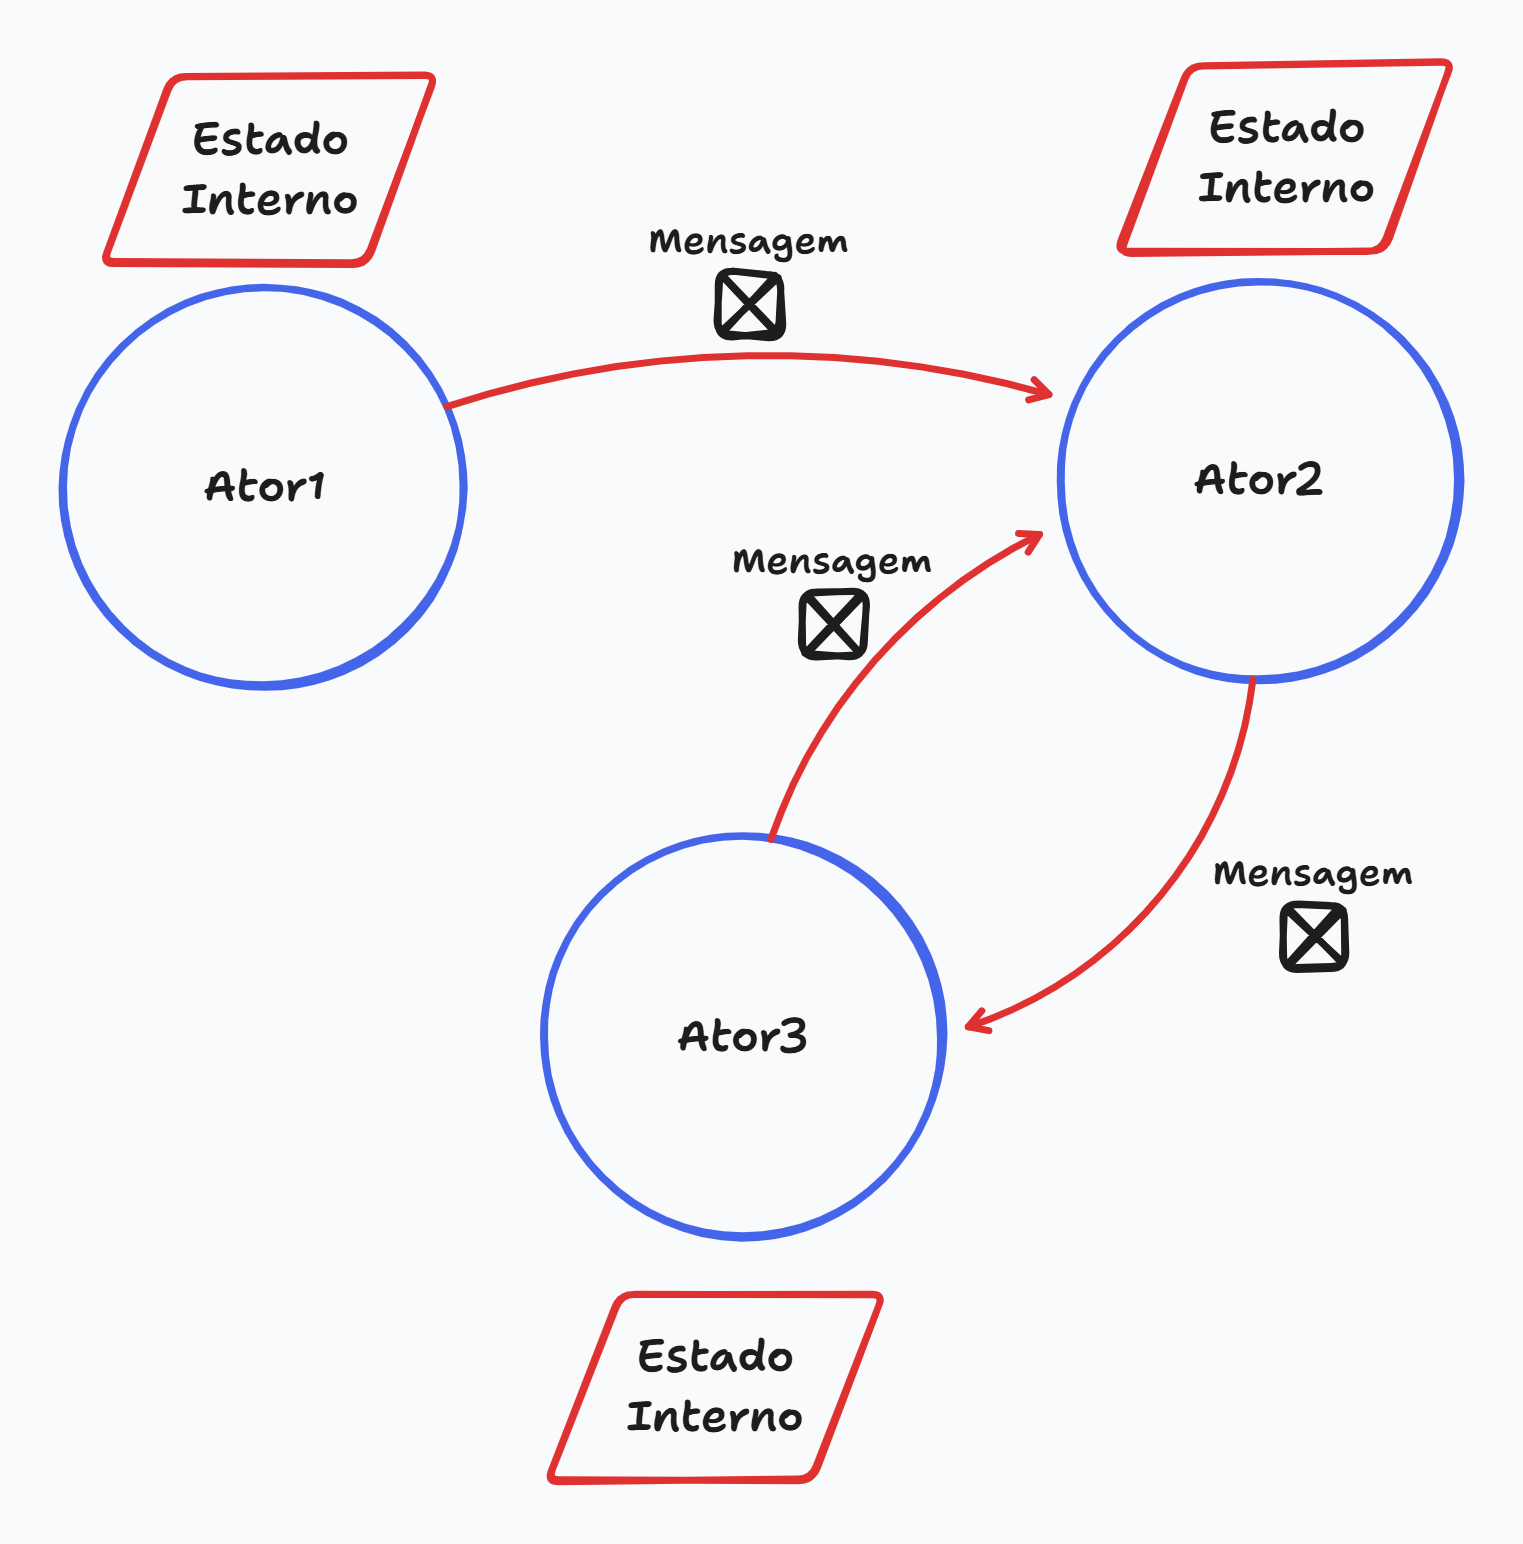
\includegraphics[width=0.6\textwidth]{figuras/actor-model.png}
        \captionof{figure}{Comunicação entre atores}
        \label{fig:actor-model}
    \end{center}
    
}


%%%%%%%% Objetivo %%%%%%%%

\posterbox[adjusted title = Objetivo, smallmargins, equal height group = toprow, colback=white, before upper=\justifying]
          {name=objetivo, below=titlebox, column=7, span=6}{

    \noindent Este trabalho realiza uma experimentação aplicando o Modelo de Atores em um contexto distante do seu domínio natural: \textbf{aplicações centralizadas em Rust}.\\

    \noindent O objetivo é entender o esforço necessário para aplicar um padrão arquitetural fora do seu contexto natural e quais consequências isso traz para o projeto.

    \begin{center}
        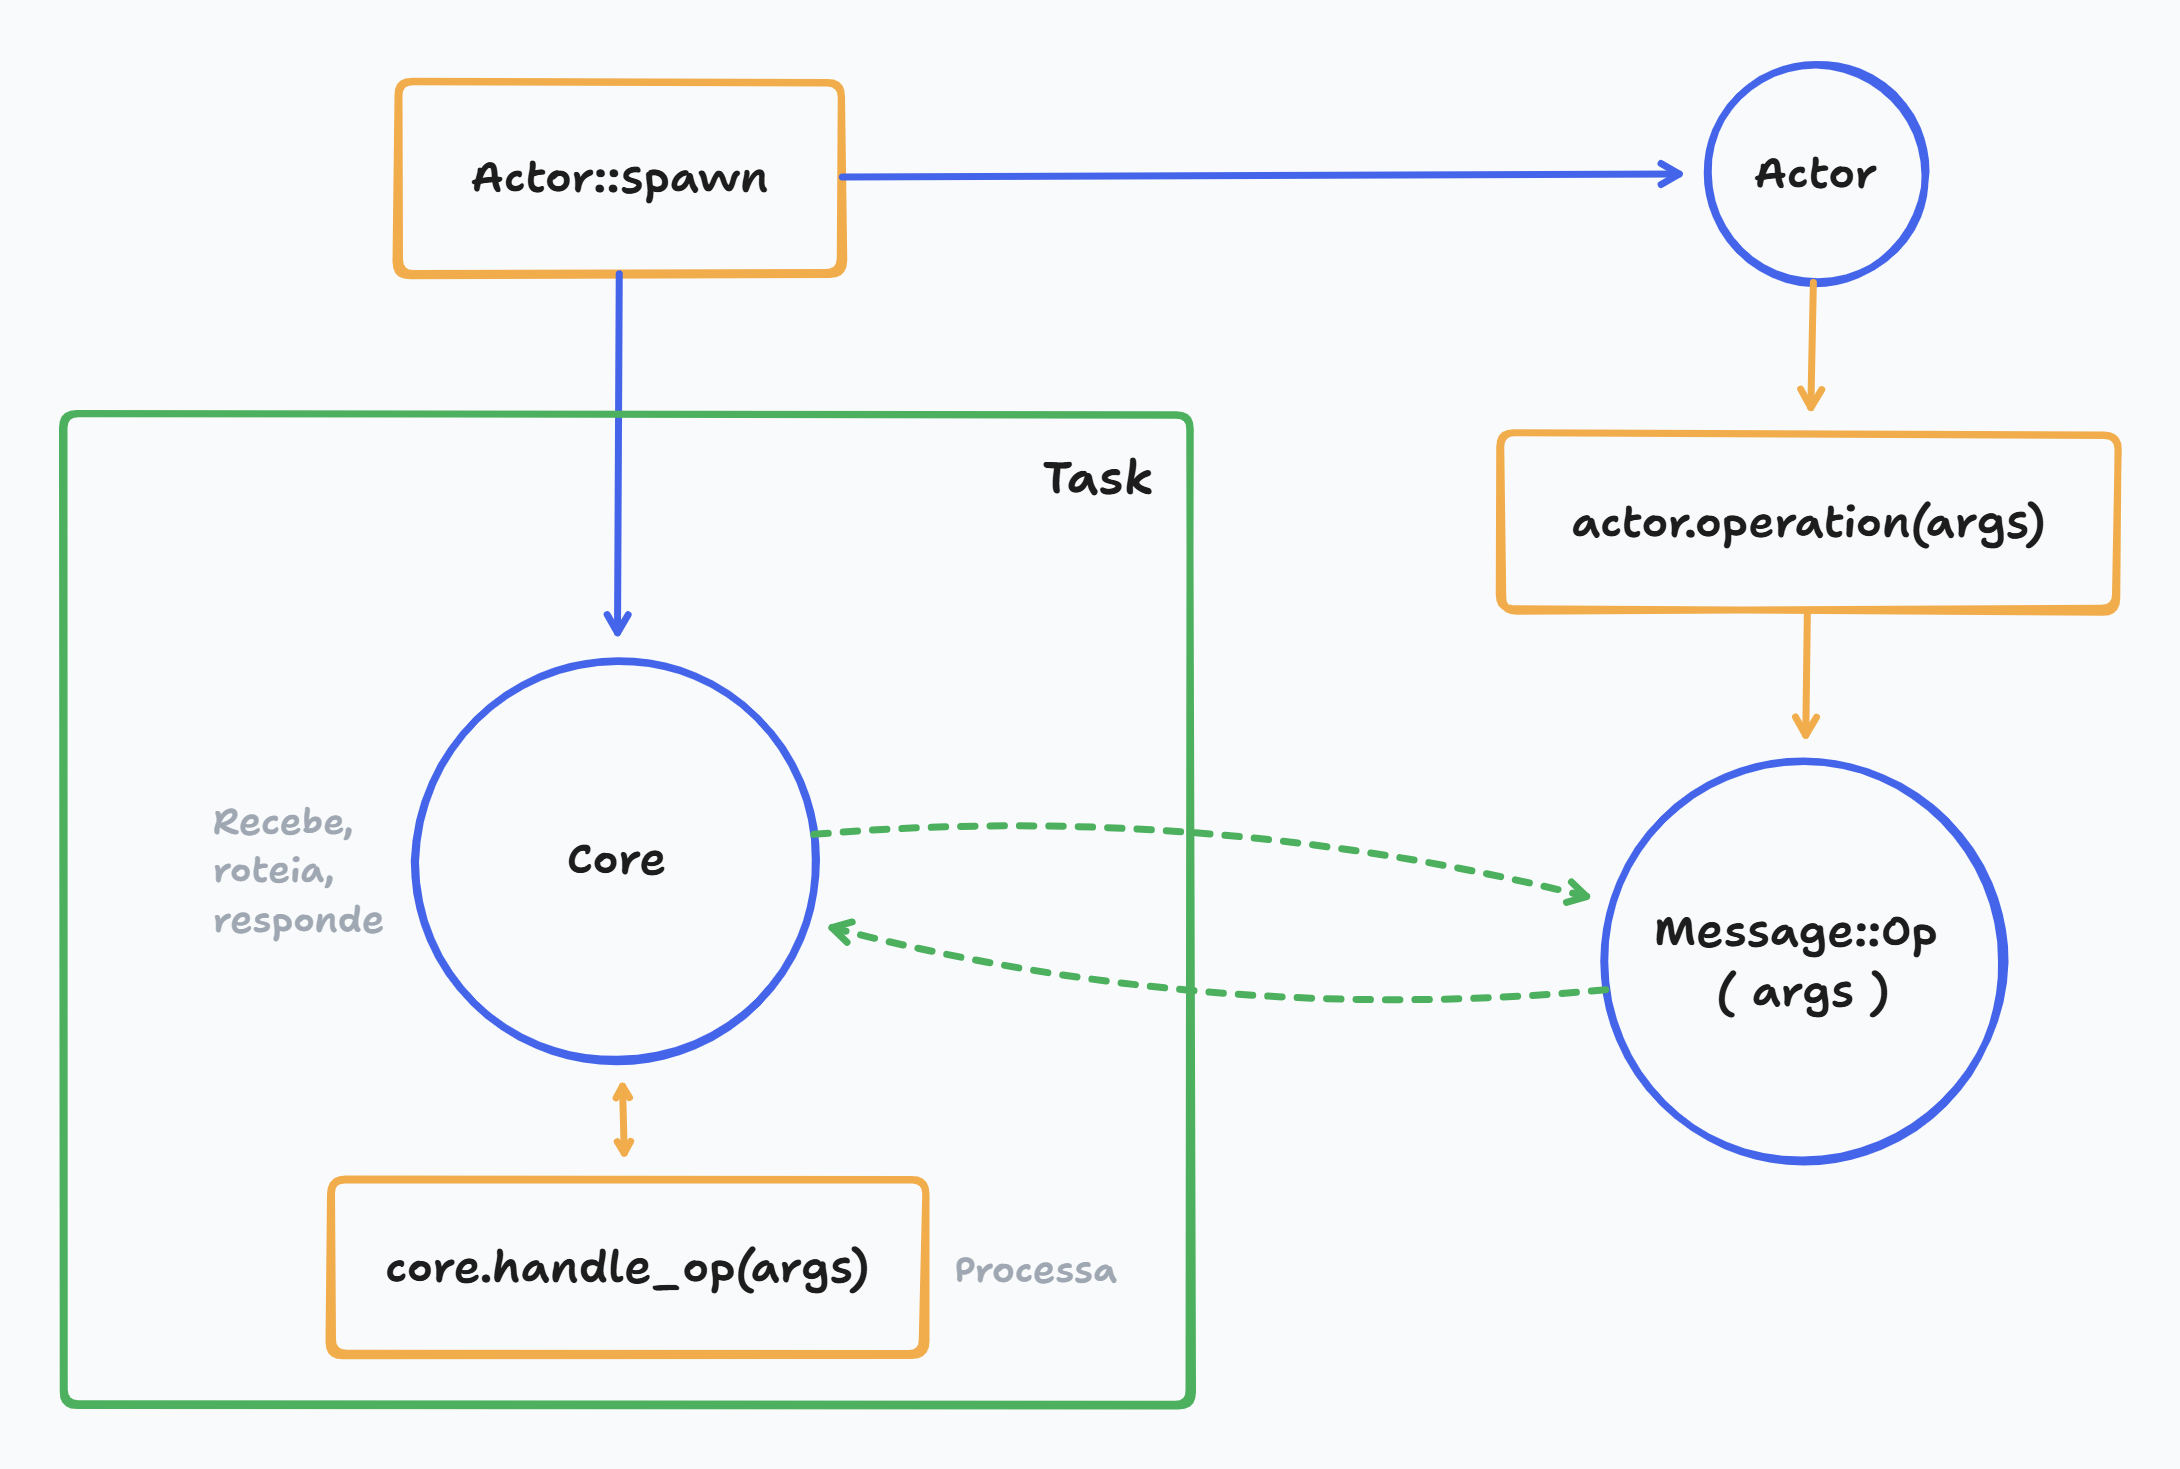
\includegraphics[width=0.6\textwidth]{figuras/actor-design.png}
        \captionof{figure}{Representação da estrutura de um ator em Rust}
        \label{fig:actor-design}
    \end{center}
}


%%%%%%%% Estudo de Caso: Patch-Hub %%%%%%%%

\posterbox[adjusted title = Estudo de Caso: \texttt{patch-hub}, smallmargins, colback=white, before upper=\justifying]
          {name=estudocaso, below=contexto, column=1, span=12}{

    \noindent\texttt{patch-hub} é uma ferramenta de terminal desenvolvida como parte do ecossistema \texttt{kworkflow} para interagir com a API do Lore Kernel Archive. Para validação, foi realizada uma reescrita do projeto aplicando o Modelo de Atores com as adaptações propostas.

    \begin{center}
    \begin{minipage}{0.48\textwidth}
        \centering
        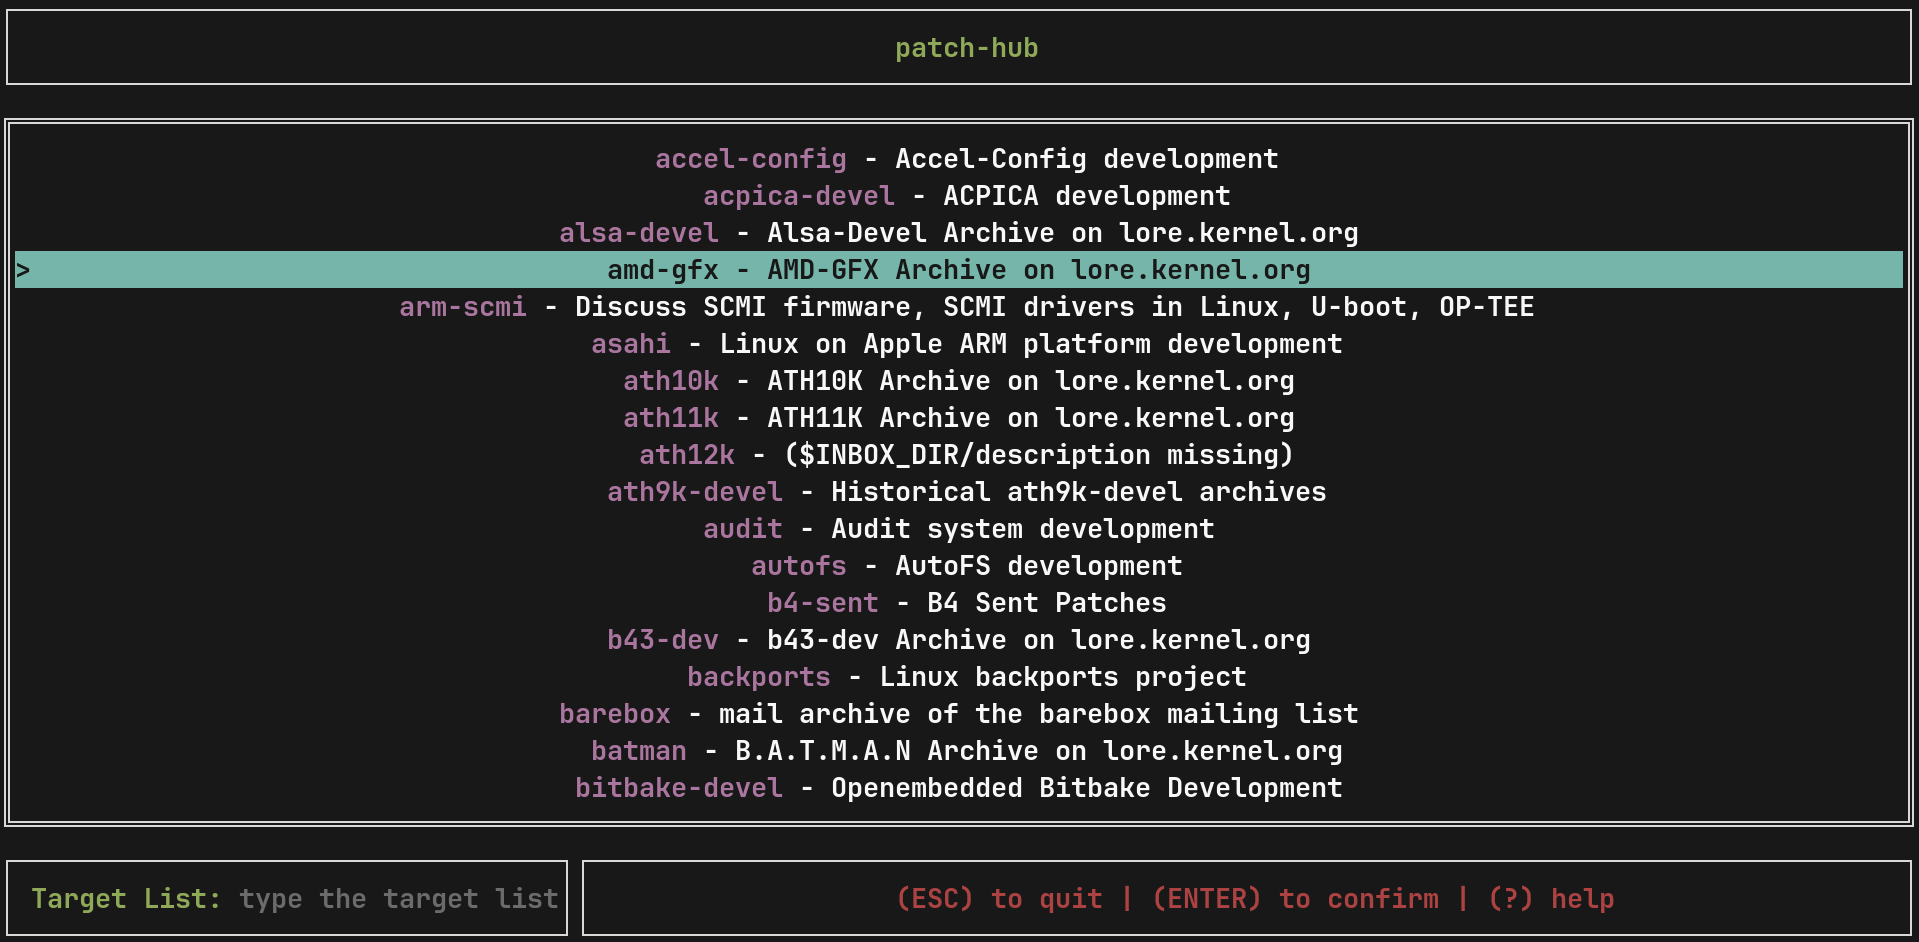
\includegraphics[width=\linewidth]{figuras/patch-hub-original.png}
        \captionof{figure}{patch-hub original}
        \label{fig:patch-hub-original}
    \end{minipage}
    \hfill
    \begin{minipage}{0.48\textwidth}
        \centering
        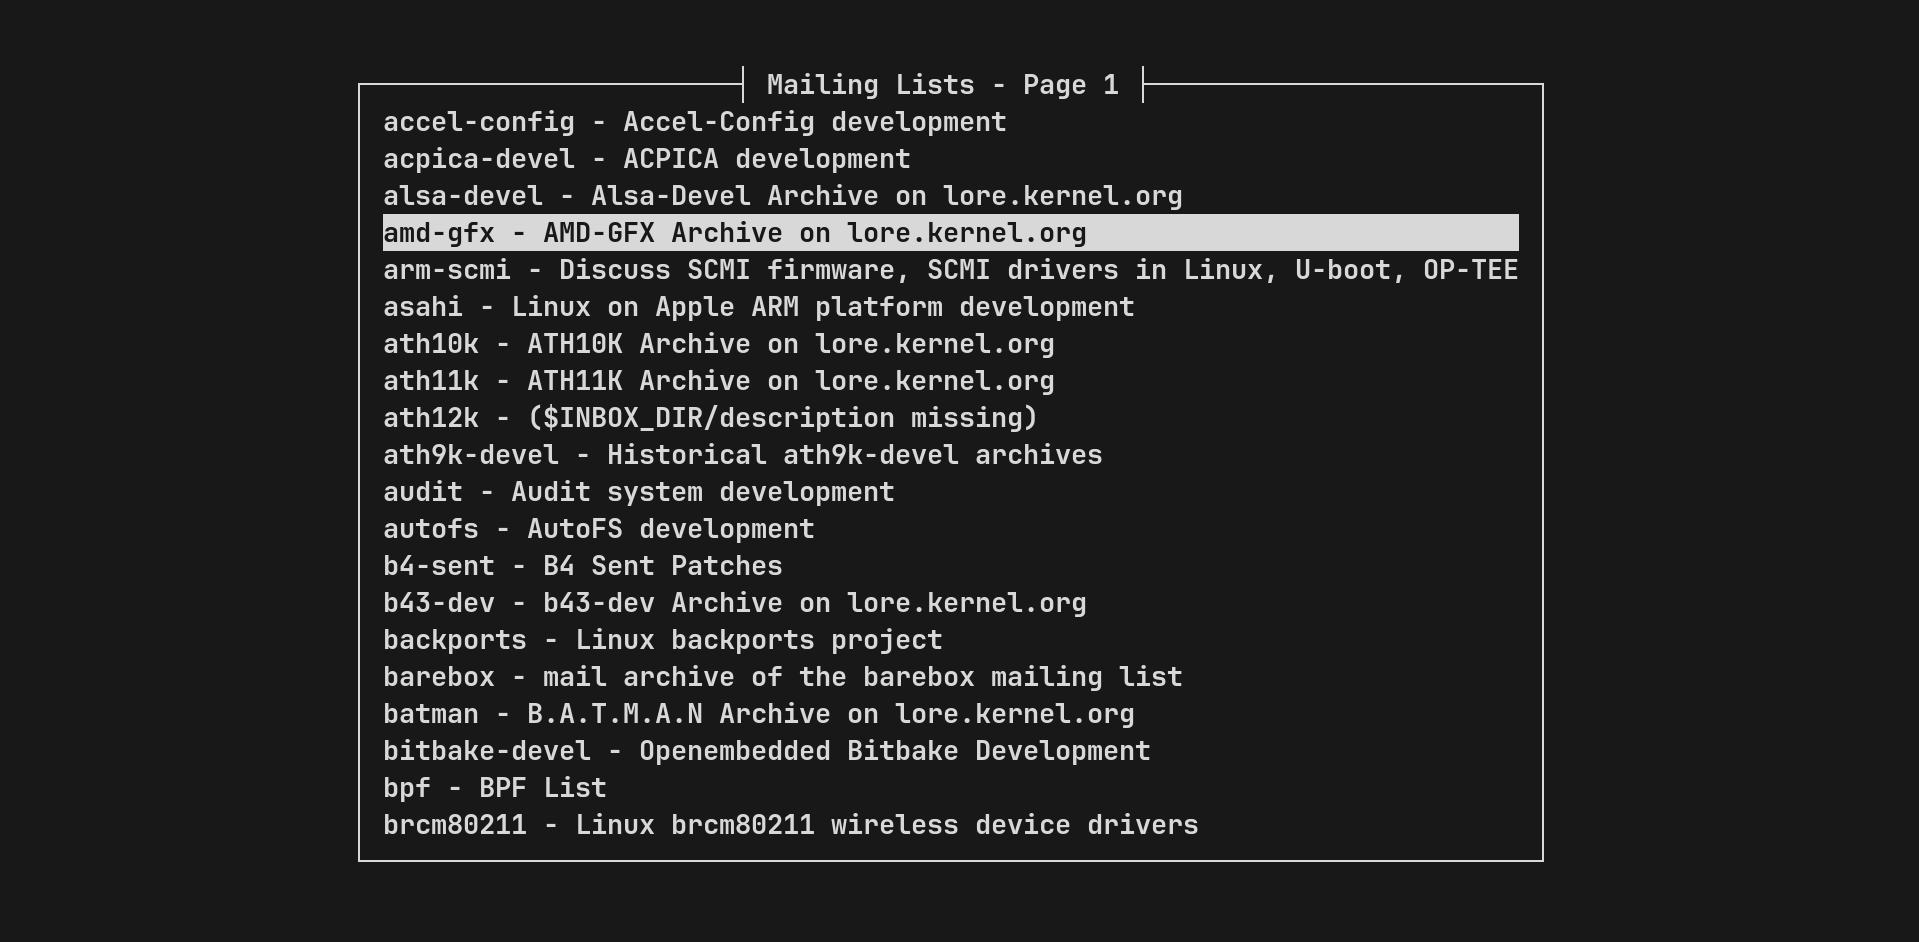
\includegraphics[width=\linewidth]{figuras/patch-hub-new.png}
        \captionof{figure}{patch-hub reescrito}
        \label{fig:patch-hub-reescrito}
    \end{minipage}
    \end{center}
}


%%%%%%%% Espaço para Imagem %%%%%%%%

\posterbox[adjusted title = Arquitetura, smallmargins, colback=white, before upper=\justifying]
          {name=arquitetura, below=estudocaso, column=1, span=5}{
    \begin{center}
        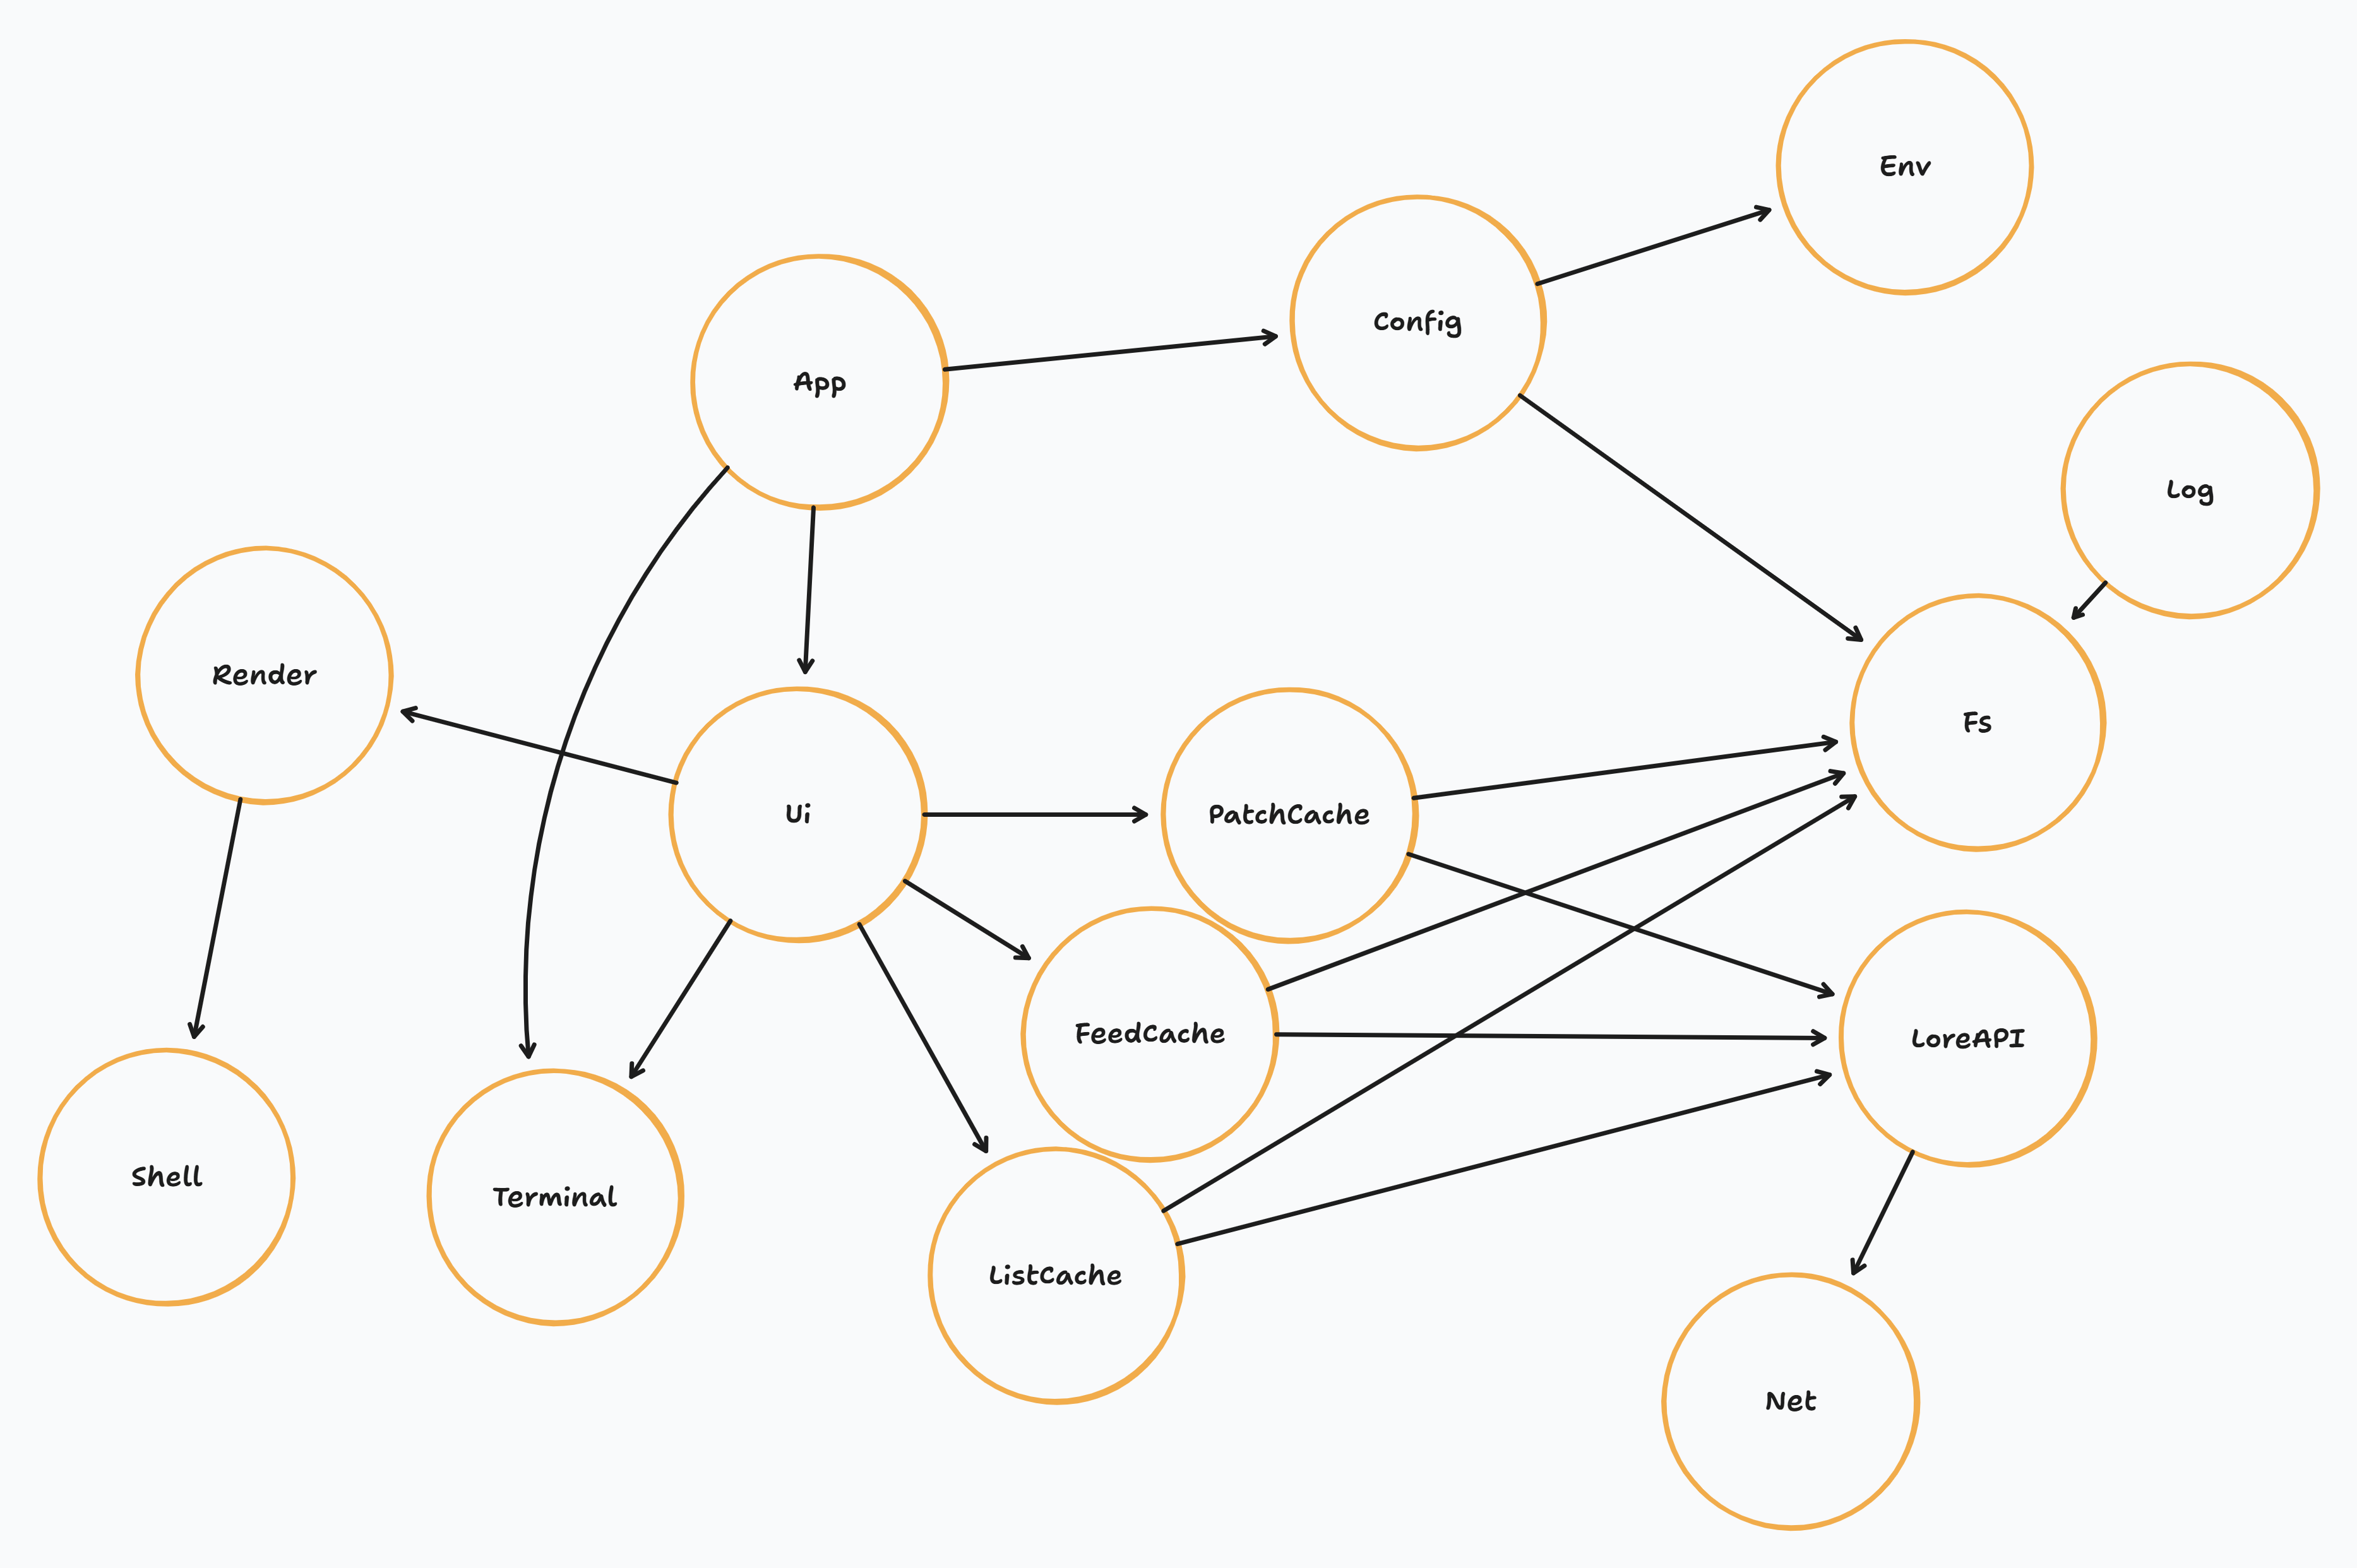
\includegraphics[width=0.92\textwidth]{figuras/patch-hub-actors.png}
        \captionof{figure}{Arquitetura do patch-hub usando atores}
        \label{fig:patch-hub-actors}
    \end{center}
}
%%%%%%%% Resultados %%%%%%%%

\posterbox[adjusted title = Resultados, smallmargins, colback=white, before upper=\justifying]
          {name=resultados, below=estudocaso, column=6, span=7}{
    \begin{itemize}
        \item \textbf{Testabilidade:} A cobertura de testes aumentou cerca de \(3x\).
        \item \textbf{Extensibilidade:} Adição de novos atores e mensagens é simples, sem necessidade de grandes modificações.
        \item \textbf{Complexidade:} A base de código aproximadamente \textbf{dobrou} de tamanho.
    \end{itemize}
}


%%%%%%%% Conclusão %%%%%%%%

\posterbox[adjusted title = Conclusão, smallmargins, colback=white, before upper=\justifying]
          {name=conclusao, below=resultados, column=6, span=7}{

    \noindent O principal resultado demonstra que a adequação de padrões arquiteturais pode ser \textbf{surpreendentemente flexível}. Sendo possível extrair valor ao se reimaginar tanto o problema quanto o padrão.
}

\end{tcbposter}

\end{document}
